\documentclass{article}
\usepackage{ae,aecompl}
\usepackage{todonotes}
\usepackage{chngcntr}
\usepackage{tikz-cd}
\usepackage{graphicx}
\graphicspath{ {./images/}}
\usepackage[all,cmtip]{xy}
\usepackage{amsmath, amscd}
\usepackage{amsthm}
\usepackage{amssymb}
\usepackage{amsfonts}
\usepackage{bm}
\usepackage{qsymbols}
\usepackage{latexsym}
\usepackage{mathrsfs}
\usepackage{mathtools}
\usepackage{cite}
\usepackage{color}
\usepackage{url}
\usepackage{enumerate}
\usepackage{verbatim}
\usepackage[draft=false, colorlinks=true]{hyperref}
\usepackage{pdfpages}
\usepackage[margin=1.2in]{geometry}
\usepackage{IEEEtrantools}

\usepackage{fancyhdr}


\usepackage[nameinlink]{cleveref}


\DeclareMathOperator*{\ac}{accept}
\DeclareMathOperator*{\amax}{argmax}
\DeclareMathOperator*{\amin}{argmin}
\DeclareMathOperator*{\Aut}{Aut}
\newcommand {\al}{{\alpha}}
\newcommand {\abs}[1]{{\left\lvert#1\right\rvert}}
\newcommand {\A}{{\mathcal{A}}}
\newcommand {\AM}{{\mathrm{AM}}}
\newcommand {\AMp}{{\AM_{p}^{X}\!(\Ri_\w)}}
\newcommand {\B}{{\mathcal{B}}}
\DeclareMathOperator*{\Be}{Bern}
\newcommand {\Br}{{\dot{B}}}
\newcommand {\Ba}{{\mathfrak{B}}}
\newcommand {\C}{{\mathbb C}}
\newcommand {\ce}{\mathrm{c}}
\newcommand {\Ce}{\mathrm{C}}
\newcommand {\Cc}{\mathrm{C_{c}}}
\newcommand {\Ccinf}{\mathrm{C_{c}^{\infty}}}
\DeclareMathOperator{\cov}{Cov}
\DeclareMathOperator{\DEV}{DEV}
\newcommand {\Di}{{\mathbb D}}
\newcommand {\dom}{\mathrm{dom}}
\newcommand{\dist}{\stackrel{\mathrm{dist}}{=}}
\newcommand {\ud}{\mathrm{d}}
\newcommand {\ue}{\mathrm{e}}
\newcommand {\eps}{\varepsilon}
\newcommand {\veps}{\varepsilon}
\newcommand {\vrho}{{\varrho}}
\newcommand {\E}{{\mathbb{E}}}
\newcommand {\Ec}{{\mathcal{E}}}
\newcommand {\Ell}{L}
\newcommand {\Ellp}{{L_{p}[0,1]}}
\newcommand {\Ellpprime}{{L_{p'}([0,1])}}
\newcommand {\Ellq}{{L_{q}([0,1])}}
\newcommand {\Ellqprime}{{L_{q'}([0,1])}}
\newcommand {\Ellr}{L^{r}}
\newcommand {\Ellone}{{L_{1}([0,1])}}
\newcommand{\Elltwo}{{L_{2}([0,1])}}
\newcommand{\Ellinfty}{L^{\infty}}
\newcommand{\Ellinftyc}{L_{\mathrm{c}}^{\infty}}
\newcommand{\exb}[1]{\exp\left\{#1\right\}}
\DeclareMathOperator*{\Ext}{Ext}
\newcommand{\F}{{\mathcal{F}}}
\newcommand{\Fe}{{\mathbb{F}}}
\newcommand{\G}{{\mathcal{G}}}
\newcommand{\HF}{\mathcal{H}_{\text{FIO}}^{1}(\Rd)}
\newcommand{\Hr}{H}
\newcommand{\HT}{\mathcal{H}}
\newcommand{\ui}{\mathrm{i}}
\newcommand{\I}{{I}}
\newcommand{\J}{{\mathcal{J}}}
\newcommand{\id}{{\mathrm{id}}}
\newcommand{\iid}{\stackrel{\mathclap{\normalfont\mbox{iid}}}{\sim}}
\newcommand{\im}{{\text{im }}}
\newcommand{\ind}{{\perp\!\!\!\perp}}
\DeclareMathOperator*{\Int}{int}
\newcommand{\intx}{{\overline{\int_{X}}}}
\newcommand{\inte}{{\overline{\int_{\E}}}}
\newcommand{\la}{\lambda}
\newcommand{\rb}{\rangle}
\newcommand{\lb}{{\langle}}
\newcommand{\La}{\Lambda}
\newcommand{\calL}{{\mathcal{L}}}
\newcommand{\lp}{{\mathcal{L}}^{p}}
\newcommand{\lpo}{{\overline{\mathcal{L}}^{p}\!}}
\newcommand{\Lpo}{{\overline{\Ell}^{p}\!}}
\newcommand{\M}{{\mathbf{M}}}
\newcommand{\Ma}{{\mathcal{M}}}
\newcommand{\N}{{{\mathbb N}}}
\newcommand{\Na}{{{\mathcal{N}}}}
\newcommand{\norm}[1]{\left\|#1\right\|}
\newcommand{\normm}[1]{{\left\vert\kern-0.25ex\left\vert\kern-0.25ex\left\vert #1 
    \right\vert\kern-0.25ex\right\vert\kern-0.25ex\right\vert}}
\newcommand{\Om}{{{\Omega}}}
\newcommand{\one}{{{\bf 1}}}
\newcommand{\pic}{\text{Pic }}
\newcommand{\ph}{{\varphi}}
\newcommand{\Pa}{{\mathbb{P}}}
\newcommand{\Po}{{\mathcal{P}}}
\newcommand{\Q}{{\mathbb{Q}}}
\newcommand{\R}{{\mathbb R}}
\newcommand{\Rd}{{\mathbb{R}^{d}}}
\DeclareMathOperator{\rej}{reject }
\newcommand{\Rn}{{\mathbb{R}^{n}}}
\newcommand{\cR}{{\mathcal{R}}}
\newcommand{\Rad}{{\mathrm{Rad}}}
\newcommand{\ran}{{\mathrm{ran}}}
\newcommand{\Ri}{{\mathrm{R}}}
\newcommand{\supp}{{\mathrm{supp}}}
\newcommand{\Se}{\mathrm{S}}
\newcommand{\Sp}{S^{*}(\Rn)}
\newcommand{\St}{{\mathrm{St}}}
\newcommand{\Sw}{\mathcal{S}}
\newcommand{\T}{{\mathcal{T}}}
\newcommand{\ta}{{\theta}}
\newcommand{\Ta}{{\Theta}}
\newcommand{\topp}{\stackrel{p}{\to}}
\newcommand{\todd}{\stackrel{d}{\to}}
\newcommand{\toL}[1]{\stackrel{L^{#1}}{\to}} 
\newcommand{\toas}{\stackrel{a.s.}{\to}}
\DeclareMathOperator{\V}{Var}
\newcommand {\w}{{\omega}}
\newcommand {\W}{{\mathrm{W}}}
\newcommand {\Wnp}{\text{$\mathrm{W}$\textsuperscript{$n,\!p$}}}
\newcommand {\Wnpeq}{\text{$\mathrm{W}$\textsuperscript{$n\!,\!p$}}}
\newcommand {\Wonep}{\text{$\mathrm{W}$\textsuperscript{$1,\!p$}}}
\newcommand {\Wonepeq}{\text{$\mathrm{W}$\textsuperscript{$1\!,\!p$}}}
\newcommand {\X}{{\mathcal{X}}}
\newcommand {\Z}{{{\mathbb Z}}}
\newcommand {\Za}{{\mathcal{Z}}}
\newcommand {\Zd}{{\Z[\sqrt{d}]}}
\newcommand {\vanish}[1]{\relax}

\newcommand {\wh}{\widehat}
\newcommand {\wt}{\widetilde}
\newcommand {\red}{\color{red}}

% Distributions
\newcommand{\normal}{\mathsf{N}}
\newcommand{\poi}{\mathsf{Poisson}}
\newcommand{\bern}{\mathsf{Bernoulli}}
\newcommand{\bin}{\mathsf{Binomal}}
\newcommand{\multi}{\mathsf{Multinomial}}
\newcommand{\Exp}{\mathsf{Exp}}



% put your command and environment definitions here




% some theorem environments
% remove "[theorem]" if you do not want them to use the same number sequence


  \newtheorem{thrm}{Theorem}
  \newtheorem{lemma}{Lemma}
  \newtheorem{prop}{Proposition}
  \newtheorem{cor}{Corollary}

  \newtheorem{conj}{Conjecture}
  \renewcommand{\theconj}{\Alph{conj}}  % numbered A, B, C etc

  \theoremstyle{definition}
  \newtheorem{defn}{Definition}
  \newtheorem{ex}{Example}
  \newtheorem{exs}{Examples}
  \newtheorem{question}{Question}
  \newtheorem{remark}{Remark}
  \newtheorem{notn}{Notation}
  \newtheorem{exer}{Exercise}




\title{STATS300A - Lecture 12}
\author{Dominik Rothenhaeusler\\ Scribed by Michael Howes}
\date{11/01/21}

\pagestyle{fancy}
\fancyhf{}
\rhead{STATS300A - Lecture 12}
\lhead{11/01/21}
\rfoot{Page \thepage}

\begin{document}
\maketitle
\tableofcontents
\section{Setting from now on}
From now on we will be doing hypothesis testing (binary decision problems). As with estimation we will have to add constraints. The two constraints we will consider are risk bounds and unbiasedness. There is a version of equivariance used in hypothesis testing but we will not study this.
\section{Set up}
As before we have data $X \sim \Pa_\ta$ and a model $\Po = \{\Pa_\ta : \ta \in \Om \}$. We now also have a partition $\Om = \Om_0 \cup \Om_1$ where $\Om_0 \subseteq \Om$ and $\Om_1 = \Om \setminus \Om_0$. From data $X$ we wish to determine if $\ta \in \Om_0$ or $\ta \in \Om_1$. We call these statements hypotheses. We have 
\begin{align*}
    H_0 &= \text{null hypothesis: } \ta \in \Om_0,\\
    H_1 &= \text{alternative hypothesis: } \ta \in \Om_1.
\end{align*}
Our decision space $D$ is $\{\rej H_0, \ac H_0\}$. We use $0-1$ loss which we can visualize as a grid. 
\begin{center}
    \begin{tabular}{|c|c|c|}
        \hline
        &$\ta \in \Om_0$&$\ta \in \Om_1$\\
        \hline 
        $\rej H_0$&1 (Type I error)&0\\
        \hline
        $\ac H_0$&0&1 (Type II error)\\
        \hline        
    \end{tabular}
\end{center}
\begin{remark}
    In this case the loss is symmetric and a Type I error is equally as bad as a Type II error. There may be times when we wish to have an asymmetrical loss. For example if we are banning a substance that may cause cancer. In this case we might worry less about Type I error. This is because failing to ban a harmful substance is much worse than banning a harmless substance.
\end{remark}
In the context of hypotheses testing we will call decision procedures tests. We will allow for randomized tests $\delta(X,U)$ but we will use a new representation for randomized procedures.
\begin{defn}
    Given a randomized test $\delta(X,U)$, the \emph{test function} of $\delta$ is a function $\phi : \X \to [0,1]$ given by 
    \[\phi(x) = \Pa(\delta(x,U)=1). \]
    That is $\phi(x)$ is the probability that we reject $H_0$ after seeing data $x$. 
\end{defn}
Note that $\phi(x)$ does not depend on the unknown parameter $\ta$. This is because $U \ind X$ and we have fixed $x$. Given a test function $\phi$ we can construct a randomized test $\delta_\phi$ that has test function $\phi$. We define $\delta_\phi$ in the folllowing way:
\begin{itemize}
    \item If $\phi(x)=1$, then $\delta_\phi(x,U)=1$ with probability 1.
    \item If $\phi(x)=0$, then $\delta_\phi(x,U)=0$ with probability 1.
    \item If $\phi(x) \in (0,1)$, then $\delta_\phi(x,U)=1$ with probability $\phi(x)$ and $\delta_\phi(x,U)=0$ otherwise.
\end{itemize}
The advantage of test functions is that there may be multiple randomized test with the same test function. These different tests are the same from a risk/decision theoretic perspective. The test function contains all the information about the risk of a test. Thus we will work with test functions rather than working with randomized tests directly.
\begin{defn}
    The \emph{power function} of a test function $\phi$ is a function $\beta : \Om \to [0,1]$ that gives the probability that $\phi$ rejects under the distribution $\Pa_\ta$. That is,
    \[\beta(\ta) = \E_\ta[\phi(X)] = \Pa_\ta(\delta_\phi \text{ rejects } H_0). \]
\end{defn}
Note that if $\ta \in \Om_0$, then 
\[\beta(\ta) = \Pa_\ta(\delta_\phi \text{ rejects } H_0) =: \text{Type I error rate}. \]
Likewise if $\ta \in \Om_1$, then 
\[1-\beta(\ta) = 1-\Pa_\ta(\delta_\phi \text{ rejects } H_0) = \Pa_\ta(\delta_\phi \text{ accepts } H_0) =: \text{Type II error rate}.  \]
Thus an optimal test would minimize $\beta(\ta_0)$ uniformly for $\ta_0 \in \Om_0$ and maximize $\beta(\ta_1)$ uniformly for $\ta_1 \in \Om_1$. Thus there is going to be a fundamental trade off between minimizing/maximizing $\beta$ in these two different regions. Consider the below picture where we have plotted the densities $p_{\ta_0}$ and $p_{\ta_1}$ for fixed $\ta_0 \in \Om_0$ and $\ta_1\in \Om_1$. Since the two densities overlap, the two error rates (corresponding to the shaded areas) trade off against each other. 
\begin{center}
    
\includegraphics[width = \textwidth]{11_01_P1.jpg}
\end{center}
\section{Level $\al$ tests}
How do we get around this tradeoff? Like with estimation, we will constrain the set of decision procedures. 
\begin{defn}
    The \emph{size} of test function $\phi$ is 
    \[\sup_{\ta_0 \in \Om_0} \E_{\ta_0}\phi(X) \in [0,1]. \]
    Thus the size is the largest possible Type I error rate. For $\al \in [0,1]$, a test $\phi$ is said to be \emph{level $\al$} if 
    \[\sup_{\ta_0 \in \Om_0}\E_{\ta_0}\phi(X) \le \al. \]
\end{defn}
We will now constrain our class of tests to the level $\al$ tests and ask which of these tests are optimal.
\begin{defn}
    A test, $\phi$, is \emph{uniformly most powerful (UMP)} at level $\al$ if $\phi$ is a level $\al$-test and among the class of level $\al$-tests, $\phi$ maximizes the power $\beta(\ta_1)$ uniformly across all $\ta_1 \in \Om$.
\end{defn}
That is, a UMP test is a level $\al$ test $\phi$ such that for all level $\al$ tests $\phi'$ and parameters $\ta_1 \in \Om_1$, we have 
\[\beta'(\ta_1) \le \beta(\ta_1), \]
where $\beta'$ and $\beta$ are the power functions of $\phi$ and $\phi'$ respectively.
\section{Optimal simple tests}
\begin{defn}
    The hypothesis $H_0$ is called \emph{simple} if $\abs{\Om_0}=1$ and otherwise $H_0$ is called \emph{composite}. Likewise, $H_1$ is called \emph{simple} if $\abs{\Om_1}=1$ and otherwise $H_1$ is called \emph{composite}.
\end{defn}
For now suppose that both $H_0$ and $H_1$ are simple and so $\abs{\Om_0}=\abs{\Om_1}=1$. Consider the measure $\mu = \Pa_0+\Pa_1$ where $H_0: X \sim \Pa_0$ and $H_1:X \sim \Pa_1$. The measures $\Pa_0$ and $\Pa_1$ are both uniformly continuous with respect to $\mu$ and thus, by Radon-Nikodym they have densities $p_0$ and $p_1$ with respect to $\mu$. Thus without loss of generality we can assume that $\Pa_0$ and $\Pa_1$ have densities with respect to a common measure.

Our goal thus becomes the constrained maximization problem 
\[\max_\phi \E_{p_1}[\phi(X)], \text{ s.t } \E_{p_0}[\phi(X)] \le \al. \]
In the case of simple testing, the maximizing test is called \emph{most powerful (MP)}.
\begin{thrm}
    \emph{[Neyman-Pearson Lemma (NPL)]} Let $\Pa_0$ and $\Pa_1$ be probability distributions with densities $p_0$ and $p_1$ w.r.t to $\mu$ and consider testing $H_0 : X \sim \Pa_0$ against $H_1 : X \sim \Pa_1$. Then,
    \begin{enumerate}
        \item[1.] \underline{Existence} there exists a test of $H_0$ against $H_1$ and a constant $k$ such  that\begin{enumerate}
            \item[(a)] $\E_{\Pa_0}\phi(X) = \al$.
            \item[(b)] $\phi(x) = \begin{cases}
                1 & \text{if } \frac{p_1(x)}{p_0(x)} > k,\\
                0 & \text{if } \frac{p_1(x)}{p_0(x)} < k.
            \end{cases}$
        \end{enumerate} 
        \item[2.] \underline{Sufficiency} If a test $\phi$ satisfies (a) and (b), then $\phi$ is MP for testing $H_0$ against $H_1$.
        \item[3.] \underline{Necessity} If $\phi$ is MP at level $\al$ for $H_0$ vs $H_1$, then $\phi$ satisfies (b) for some $k \in [0,\infty]$. The test $\phi$ also satisfies (a) unless there exists a test with size strictly smaller than $\al$ and power equal to 1 for all $\ta_1 \in \Om_1$. 
    \end{enumerate}
\end{thrm}
Note that in 1.(b) we do not specify the value of $\phi(x)$ when $\frac{p_1(x)}{p_2(x)} = k$. We will discuss this case during the proof. The condition in part 3. where (a) does not hold is rather rare. It corresponds to when we have a rejection region which contains the entire support of $p_1$ and $p_0$ has probability less than $\al$ of lying in said region. Thus our densities look like one of the below pictures

\begin{center}
    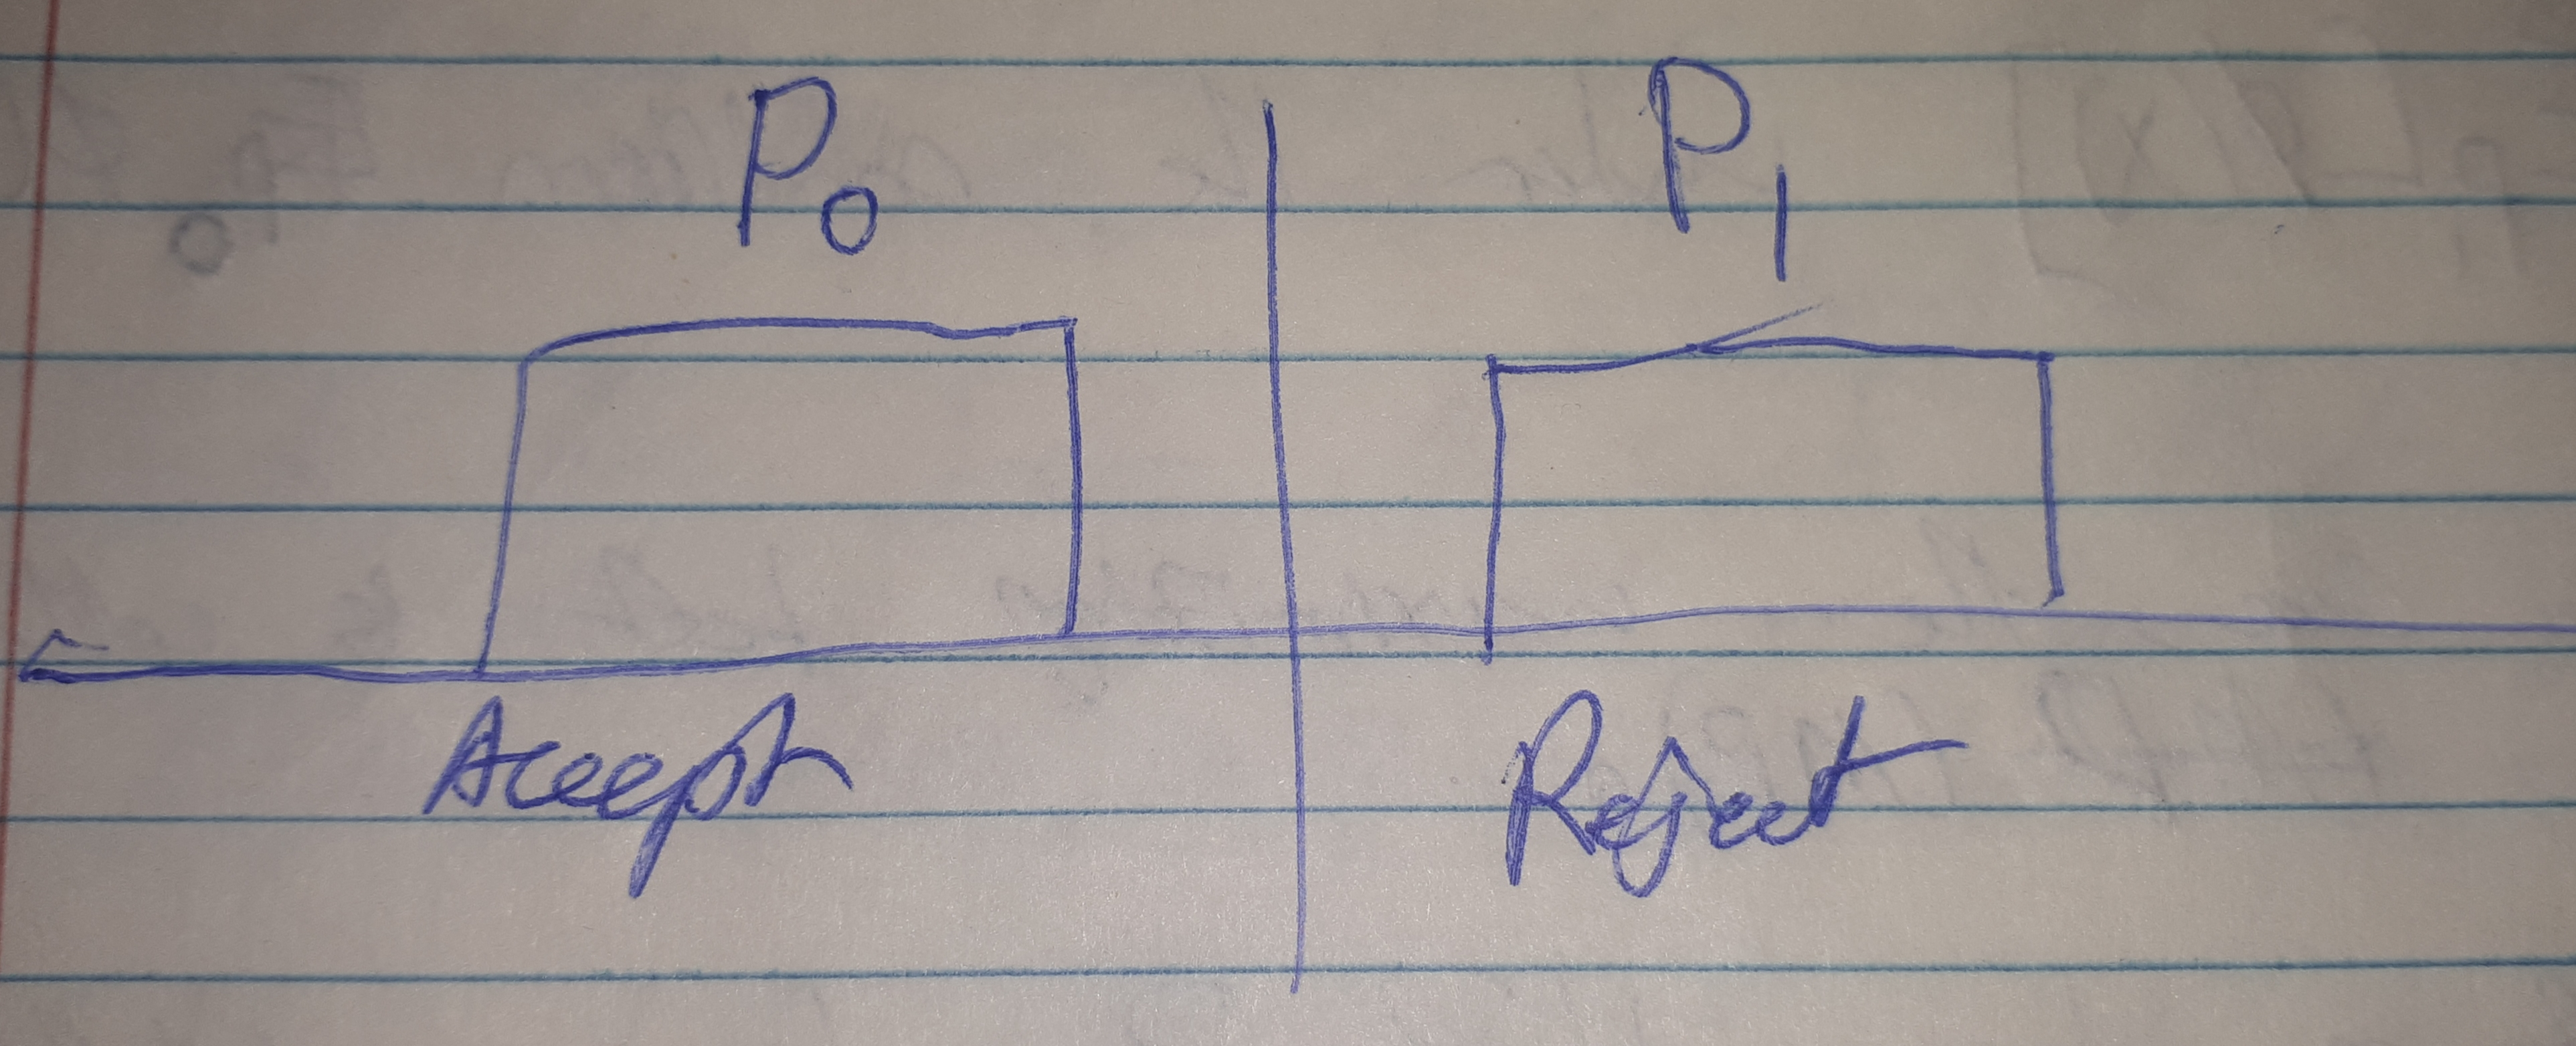
\includegraphics[width = \textwidth]{11_01_P2.jpg}

    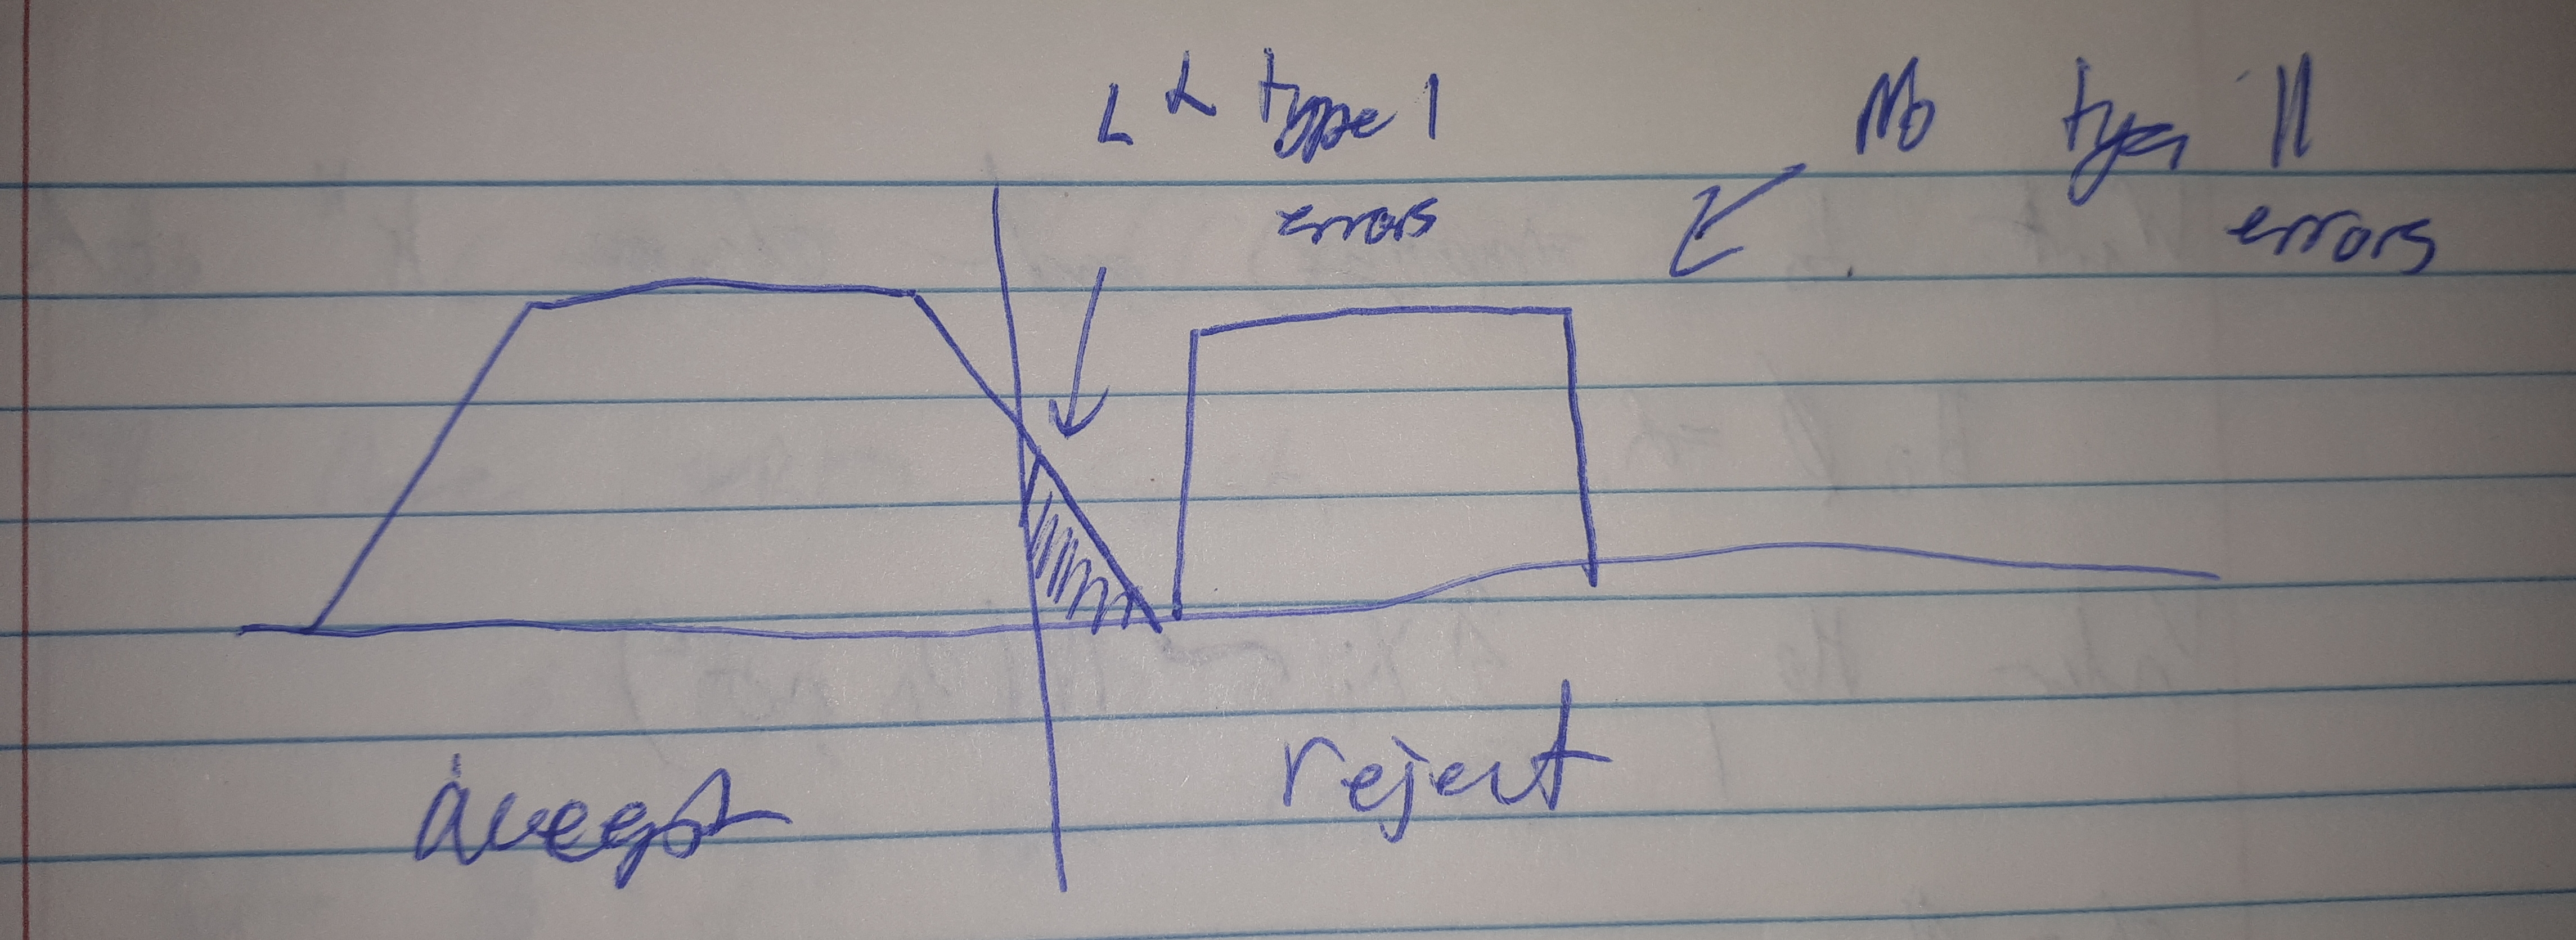
\includegraphics[width = \textwidth]{11_01_P3.jpg}
\end{center}

In both of these cases the problem of hypothesis testing at level $\al$ has become somewhat trivial.

\begin{ex}
    Here we discuss a continuous example. For a discrete example - see the scribed notes. Suppose our data is $X_1,\ldots, X_n \sim \Na(\mu,\sigma^2)$ where $\sigma^2$ is known. Consider the hypotheses $H_0 : \mu = 0$ and $H_1 : \mu = \mu_1$ where $\mu_1 > 0$. By NPL we can find the most powerful test by looking at the likelihood ration. Note that
    \begin{align*}
        r(x) &= \frac{p_1(x)}{p_0(x)}\\
        &= \frac{\prod_{i=1}^n \frac{1}{\sqrt{2\pi}\sigma}\exb{-\frac{1}{2\sigma^2}\left(x_i-\mu_1\right)^2}}{\prod_{i=1}^n \frac{1}{\sqrt{2\pi}\sigma}\exb{-\frac{1}{2\sigma^2}x_i^2}}.
    \end{align*}
    Thus $r(x) > k$ if and only if $\log(r(x)) > k'$ if and only if $\sum_{i=1}^n x_i > k''$. We wish to choose $k''$ such that 
    \[\Pa_0\left(\sum_{i=1}^n X_i > k''\right) =\E_0\phi = \al. \]
    Under $H_0$ we know that $\sum_{i=1}^n X_i \sim \Na(0,n\sigma^2)$. Thus the test $\phi = \mathbb{I}(\sum_{i=1}^n X_i > k'')$ is equivalent to $\phi = \mathbb{I}(\frac{1}{\sigma \sqrt{n}}\sum_{i=1}^n X_i > k''')$. The latter test has level $1-\Phi(k''')$ where $\Phi$ is the CDF of a $\Na(0,1)$ random variable. Thus we choose $k''' =  \Phi^{-1}(1-\al)$. Such a test satisfies (b) and (a) and thus is the MP test for the two simple hypothesis $H_0$ and $H_1$.

    However, our test $\phi$ does not depend on $\mu_1$ and thus $\phi$ is the uniformly most powerful test of $H_0 : \mu =0$ against $H_1 : \mu > 0$. (Note that the condition $\mu_1 > 0$ was important in the above calculations). This is a common strategy for find UMP tests. First restrict to simple test and then show that the MP test does not depend on the choice of parameter used for the simple test. 
    
    In this example, how we go from $k'$ to $k''$ and the power of the test depend on $\mu_1$ but the final test we constructed does not depend on $\mu_1$.
\end{ex}
\begin{proof}[Proof of Neyman Pearson]
    We will start the proof today and finish it next lecture. We will first prove existance (part 1.). Let $r(x) = \frac{p_1(x)}{p_0(x)}$ and define a function $\al(c) = \Pa_0(r(X) > c)$. If there exists $c_\al$ such that $\al = \Pa_0(r(X) > c_\al)$, then define $\phi$ by
    \[\phi(x) = \begin{cases}
        1 &\text{if } r(x) > c_\al,\\
        0 & \text{else}.
    \end{cases} \]
    Then $\phi$ satisfies (b) and 
    \[\Pa_0(\rej H_0) = \Pa_0(r(X) > c_\al) = \al.\]
    Thus $\phi$ also satisfies (a). We will continue this proof next lecture.
\end{proof}
\end{document}